\section{Конструкторский раздел}
В данном разделе представлены требования к программному обеспечению, сведения о реализуемом модуле и дополнительном программном обеспечении. Также приведены схемы, описывающие работу компонентов.

\subsection{Требования к программному обеспечению}
Требуется реализовать загружаемый модуль ядра для мониторинга приоритетов, времени выполнения и простоя процессов, который будет получать информацию о процессах в режиме ядра и предоставлять доступ к данной информации через procfs.

В целях упрощения работы с данным модулем также потребуется реализовать дополнительную программу, выполняющую загрузку модуля в систему, а также предоставляющую получаемую из procfs информацию без дополнительных манипуляций пользователя.

\subsection{Модуль логирования процессов реального времени}
Для хранения информации о приоритетах, времени выполнения и простоя процессов реального времени выделяется массив символов.

\begin{code}
	\captionof{listing}{Массив символов журнала.}
	\label{code:charLog}
	\inputminted
	[
	frame=single,
	framerule=0.5pt,
	framesep=20pt,
	fontsize=\small,
	tabsize=4,
	linenos,
	numbersep=5pt,
	xleftmargin=10pt,
	firstline=26,
	lastline=27,
	breaklines=true
	]
	{text}
	{code/oldMd.c}
\end{code}

Для того, чтобы не допускать переполнений при записи в журнал, каждый раз перед занесением данных в лог проверяется, может ли он в данный момент вместить новые данные.

\begin{code}
	\captionof{listing}{Функция проверки переполнения.}
	\label{code:checkOverflowFunction}
	\inputminted
	[
	frame=single,
	framerule=0.5pt,
	framesep=20pt,
	fontsize=\small,
	tabsize=4,
	linenos,
	numbersep=5pt,
	xleftmargin=10pt,
	firstline=27,
	lastline=39,
	breaklines=true
	]
	{text}
	{code/oldMd.c}
\end{code}

\begin{code}
	\captionof{listing}{Пример использования функции проверки переполнения.}
	\label{code:checkOverflowFunctionExecution}
	\inputminted
	[
	frame=single,
	framerule=0.5pt,
	framesep=20pt,
	fontsize=\small,
	tabsize=4,
	linenos,
	numbersep=5pt,
	xleftmargin=10pt,
	firstline=52,
	lastline=58,
	breaklines=true
	]
	{text}
	{code/oldMd.c}
\end{code}

Как видно из предоставленного листинга \ref{code:checkOverflowFunctionExecution} в случае обнаружения переполнения модуль не прекращает свое выполнение.

В листинге \ref{code:proc_ops_realization} приведено заполнение структуры proc\_ops. Требуется, чтобы функция yaRead включала в себя вызов функции copy\_to\_user в целях передачи информации из журнала в пространство пользователя.

\begin{code}
	\captionof{listing}{Заполнение структуры proc\_ops.}
	\label{code:proc_ops_realization}
	\inputminted
	[
	frame=single,
	framerule=0.5pt,
	framesep=20pt,
	fontsize=\small,
	tabsize=4,
	linenos,
	numbersep=5pt,
	xleftmargin=10pt,
	%firstline=52,
	%lastline=58,
	breaklines=true
	]
	{text}
	{code/proc_ops_realization.h}
\end{code}

В листинге \ref{code:initExit} предоставлены функции инициализации и завершения работы модуля.

\begin{code}
	\captionof{listing}{Функции инициализации и завершения работы модуля.}
	\label{code:initExit}
	\inputminted
	[
	frame=single,
	framerule=0.5pt,
	framesep=20pt,
	fontsize=\small,
	tabsize=4,
	linenos,
	numbersep=5pt,
	xleftmargin=10pt,
	firstline=133,
	lastline=160,
	breaklines=true
	]
	{text}
	{code/oldMd.c}
\end{code}

В данном фрагменте можно увидеть, что в функции инициализации модуля требуется запустить отдельный поток для журналирования, так как в ином случае инициализация не будет завершена до окончания выполнения требующегося количества итераций сбора информации.

\subsection{Программа загрузки модуля и получения информации}
Программа загрузки модуля и вывода полученной информации должна включать в себя два системных вызова: загрузки и выгрузки модуля. Также требуется получить доступ к файлу, создаваемому модулем в procfs. Данное действие может быть произведено с использованием вызова cat.

В листингах \ref{code:systemInsmod}--\ref{code:systemPopen} предоставлены фрагменты выполнения указанных вызовов.

\begin{code}
	\captionof{listing}{Загрузка модуля в систему.}
	\label{code:systemInsmod}
	\inputminted
	[
	frame=single,
	framerule=0.5pt,
	framesep=20pt,
	fontsize=\small,
	tabsize=4,
	linenos,
	numbersep=5pt,
	xleftmargin=10pt,
	firstline=22,
	lastline=22,
	breaklines=true
	]
	{text}
	{../../src/starterLogger.c}
\end{code}

\begin{code}
	\captionof{listing}{Выгрузка модуля из системы.}
	\label{code:systemRmmod}
	\inputminted
	[
	frame=single,
	framerule=0.5pt,
	framesep=20pt,
	fontsize=\small,
	tabsize=4,
	linenos,
	numbersep=5pt,
	xleftmargin=10pt,
	firstline=45,
	lastline=45,
	breaklines=true
	]
	{text}
	{../../src/starterLogger.c}
\end{code}

\begin{code}
	\captionof{listing}{Выполнения вызова cat.}
	\label{code:systemPopen}
	\inputminted
	[
	frame=single,
	framerule=0.5pt,
	framesep=20pt,
	fontsize=\small,
	tabsize=4,
	linenos,
	numbersep=5pt,
	xleftmargin=10pt,
	firstline=26,
	lastline=32,
	breaklines=true
	]
	{text}
	{../../src/starterLogger.c}
\end{code}

Функция popen в листинге \ref{code:systemPopen} открывает процесс, создавая канал, производя fork и вызывая командную оболочку. Возвращаемое значение данный функции -- это поток ввода-вывода. При этом будет возвращен NULL, если вызовы fork или pipe завершились ошибкой или если невозможно выделить необходимый для этого объем памяти.

\subsection{Схемы работы модуля и дополнительного программного обеспечения}
На рисунках \ref{fig:init}--\ref{fig:starterLogger} предоставлены схемы работы модуля и дополнительного программного обеспечения.

\begin{figure}[H]
	\centering
	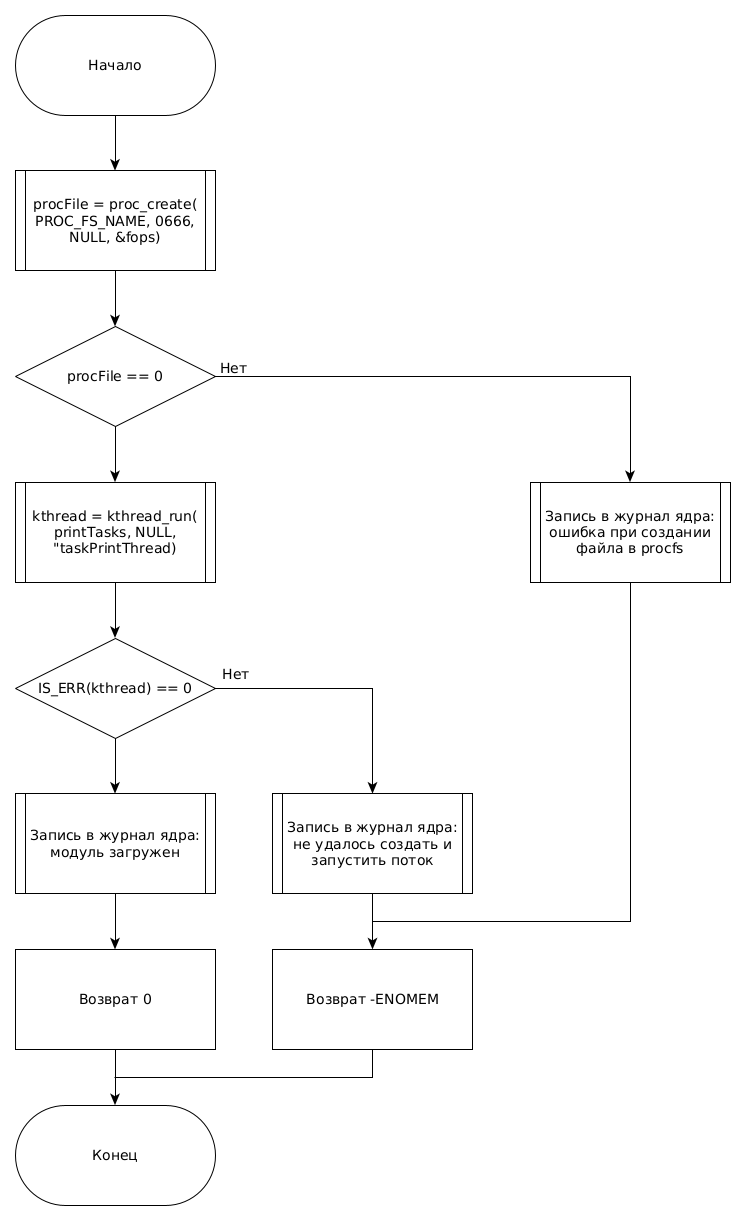
\includegraphics[scale=0.5]{img/init.png}
	\caption{Схема функции инициализации модуля.}
	\label{fig:init}
\end{figure}

\begin{figure}[H]
	\centering
	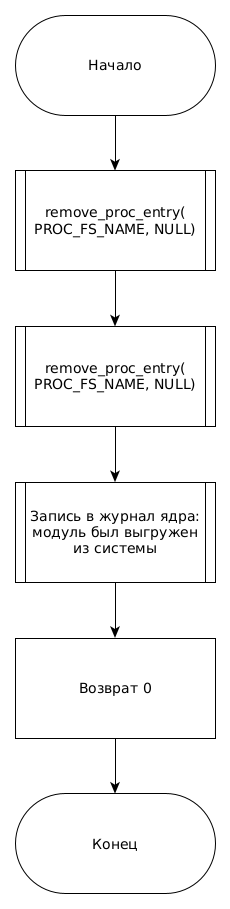
\includegraphics[scale=0.5]{img/exit.png}
	\caption{Схема функции завершения работы модуля.}
	\label{fig:exit}
\end{figure}

\begin{figure}[H]
	\centering
	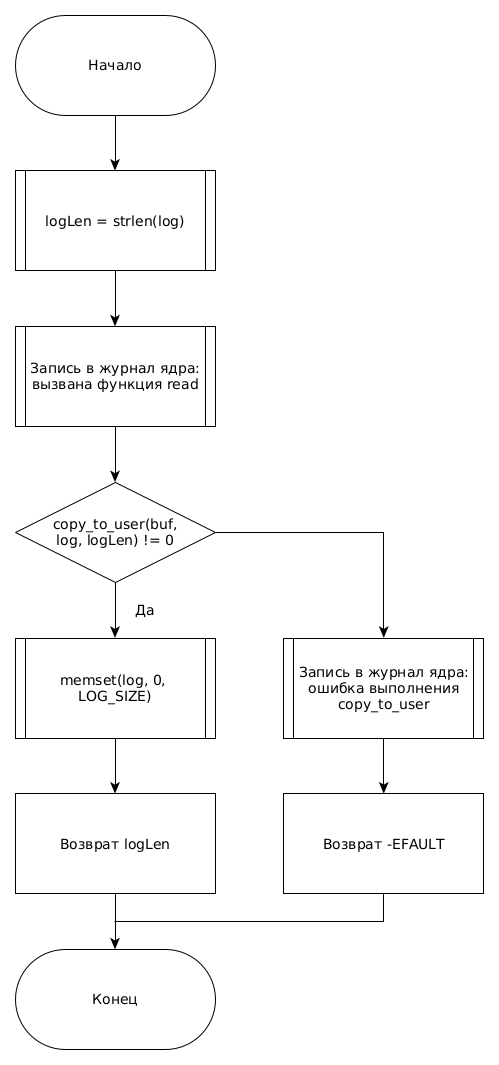
\includegraphics[scale=0.5]{img/yaRead.png}
	\caption{Схема функции yaRead обработки чтения из /proc. }
	\label{fig:read}
\end{figure}

\begin{figure}[H]
	\centering
	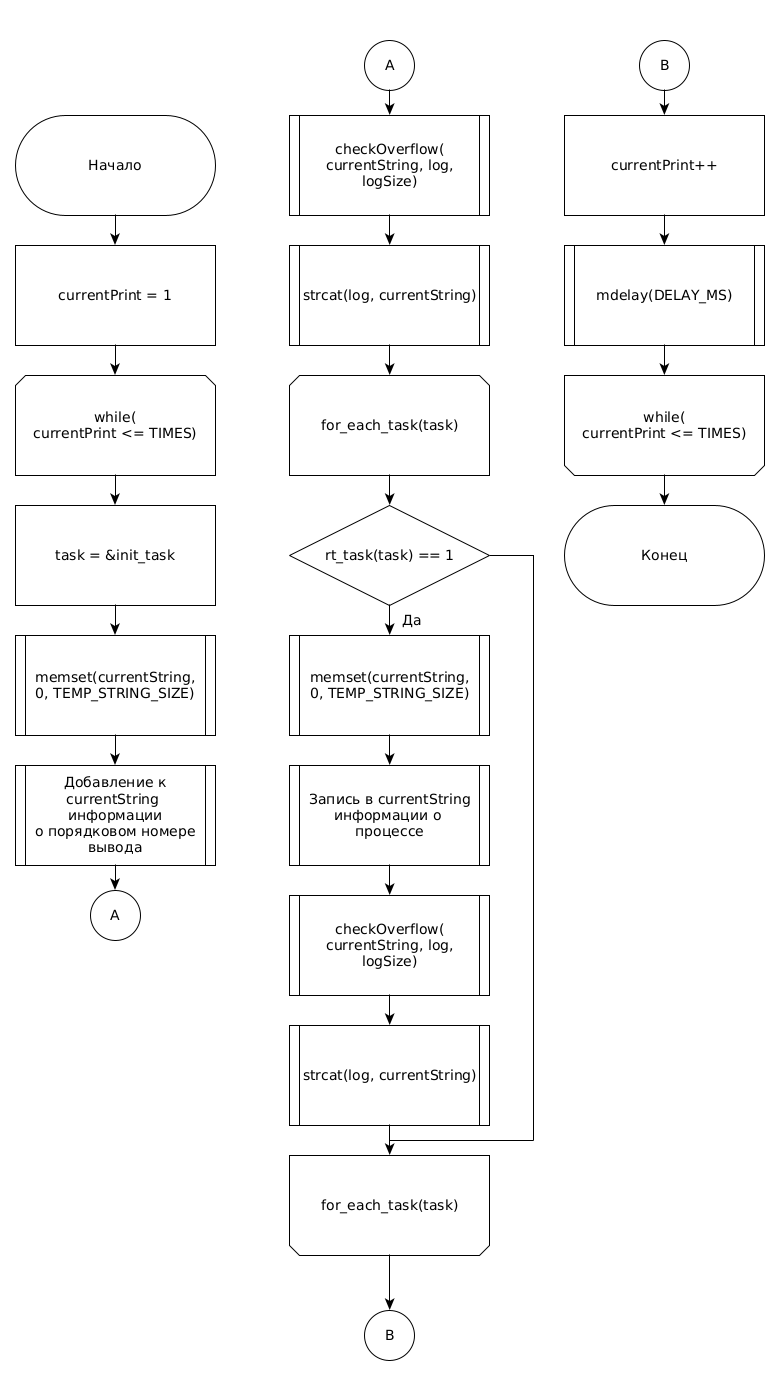
\includegraphics[scale=0.5]{img/printTasks.png}
	\caption{Схема функции printTasks вывода информации о процессах реального времени. }
	\label{fig:printTasks}
\end{figure}

\begin{figure}[H]
	\centering
	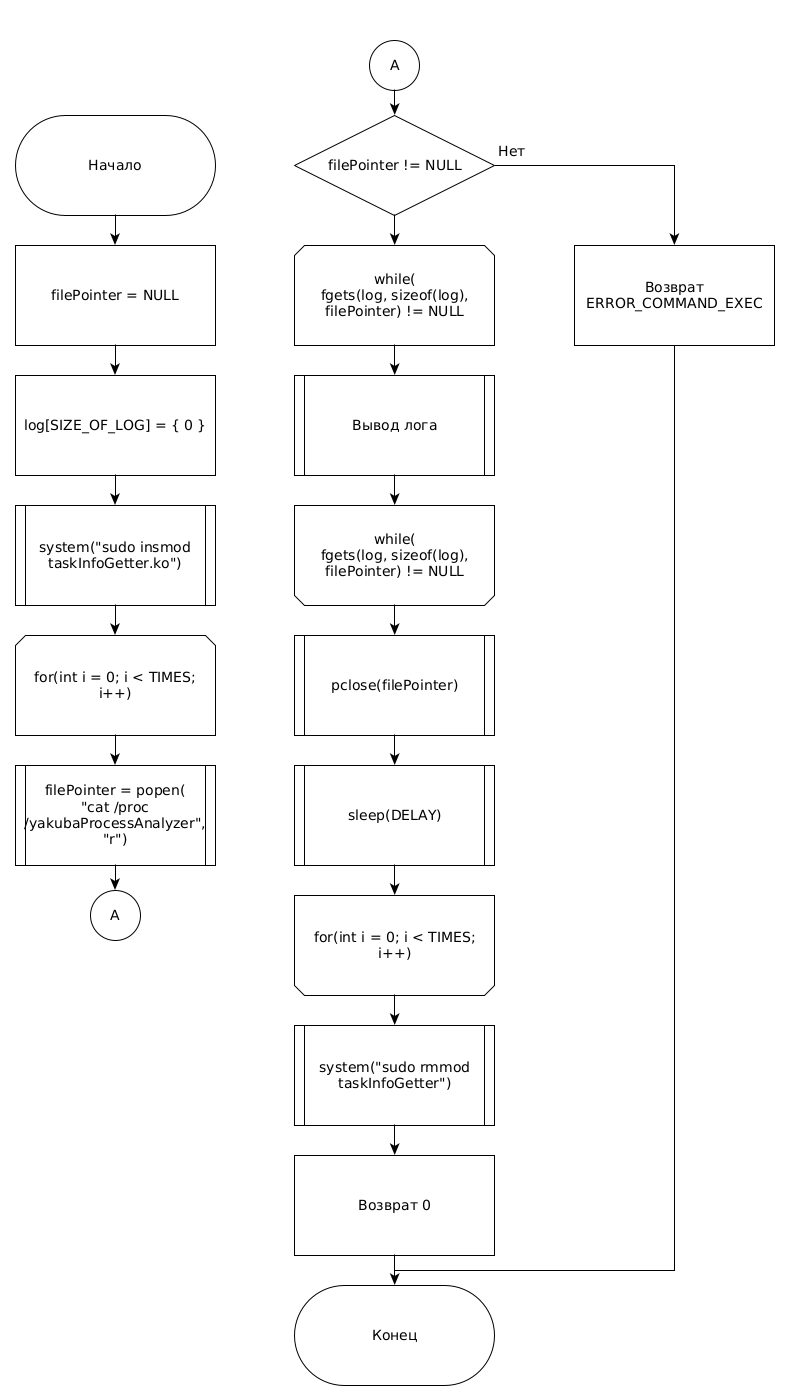
\includegraphics[scale=0.5]{img/starterLogger.png}
	\caption{Схема работы программы загрузки модуля и получения информации. }
	\label{fig:starterLogger}
\end{figure}

\subsubsection*{Вывод}
В разделе были представлены требования к программному обеспечению. Было обозначено, что требуется реализовать загружаемый модуль ядра для мониторинга приоритетов, времени выполнения и простоя процессов. Также было решено реализовать дополнительную программу загрузки модуля в систему и вывода лога.

Были приведены основные сведения о компонентах, а также схемы, описывающие их работу.

\pagebreak